\hebrewsection{Digital Communication Systems}

\subsection{Introduction to Digital Communication}
Digital communication systems transmit discrete messages over physical channels. The main advantages over analog systems are noise immunity, ease of multiplexing, and the ability to use error correction.

\subsection{Signal Space Concepts}
In signal space theory, waveforms are represented as vectors in an $N$-dimensional space. This geometric representation simplifies the analysis of modulation performance.

\subsection{Pulse Shaping and the Nyquist Criterion}
To transmit symbols at a rate $1/T$ without Inter-Symbol Interference (ISI), the pulse $p(t)$ must satisfy the Nyquist Criterion.

\subsubsection{Raised Cosine Filter}
The Raised Cosine (RC) filter is the standard for pulse shaping. It minimizes ISI by having zero-crossings at symbol intervals.
\begin{equation}
    P(f) = \begin{cases} T & |f| \leq \frac{1-\alpha}{2T} \\ \dots & \dots \end{cases}
\end{equation}
where $\alpha$ is the \textbf{roll-off factor}.

\subsubsection{Root Raised Cosine (RRC) Filter}
In practical systems, the RC filter is split between the transmitter and the receiver. Each uses an RRC filter:
\begin{equation}
    H_{TX}(f) = H_{RX}(f) = \sqrt{P(f)}
\end{equation}
This ensures that the combined response is RC, and the receiver filter is matched to the transmitted pulse, maximizing the SNR.

\subsection{Modulation Schemes}
\subsubsection{M-ary Phase Shift Keying (M-PSK)}
Phase is modulated among $M$ discrete values. Constant envelope makes it suitable for non-linear power amplifiers.

\subsubsection{Quadrature Amplitude Modulation (QAM)}
QAM varies both amplitude and phase, providing high spectral efficiency.
\begin{equation}
    s(t) = I(t)\cos(2\pi f_c t) - Q(t)\sin(2\pi f_c t)
\end{equation}
QAM is the foundation for modern high-speed wireless (Wi-Fi 6 uses 1024-QAM).

\subsection{Continuous Phase Modulation (CPM)}
CPM is a memory-based modulation where the phase is constrained to be continuous. This results in very low spectral sidelobes.

\subsubsection{Gaussian Minimum Shift Keying (GMSK)}
GMSK is a specific form of CPM where the frequency pulses are shaped by a Gaussian filter. It was the standard for GSM cellular systems due to its spectral efficiency and constant envelope.

\begin{center}
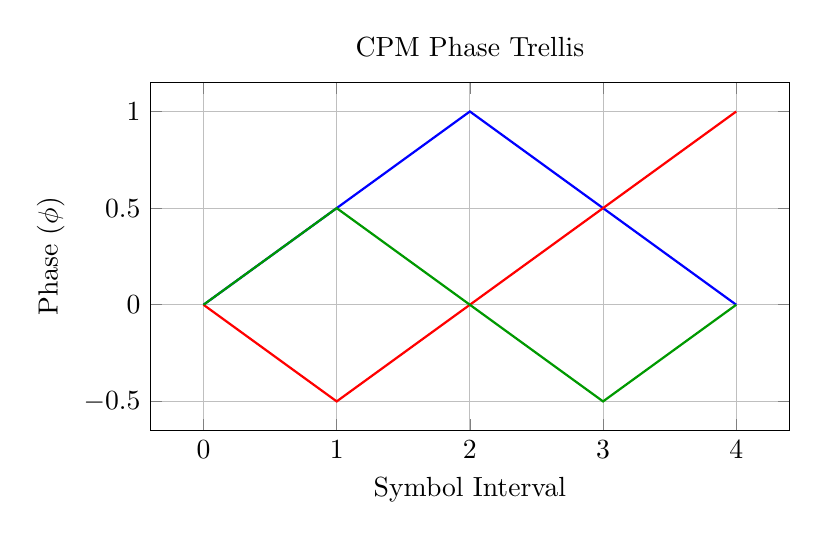
\begin{tikzpicture}
\begin{axis}[
    title={CPM Phase Trellis},
    xlabel={Symbol Interval},
    ylabel={Phase ($\phi$)},
    grid=major,
    width=0.8\textwidth,
    height=6cm
]
\addplot[blue, thick] coordinates {(0,0) (1,0.5) (2,1) (3,0.5) (4,0)};
\addplot[red, thick] coordinates {(0,0) (1,-0.5) (2,0) (3,0.5) (4,1)};
\addplot[green!60!black, thick] coordinates {(0,0) (1,0.5) (2,0) (3,-0.5) (4,0)};
\end{axis}
\end{tikzpicture}
\end{center}

\subsection{Carrier and Symbol Synchronization}
The receiver must recover the carrier frequency and phase.
\subsubsection{The Costas Loop}
The Costas loop is a standard method for carrier phase recovery in BPSK and QPSK. it uses two branches (I and Q) to generate an error signal that drives a Voltage Controlled Oscillator (VCO).

\subsubsection{Symbol Timing Recovery}
Algorithms like the \textbf{Mueller-Müller} or \textbf{Gardner} detectors are used to sample the received signal at the optimal instant.

\subsection{Equalization}
Equalizers combat channel-induced ISI. \textbf{Zero-Forcing (ZF)} and \textbf{Minimum Mean Square Error (MMSE)} are common linear equalizers. \textbf{Decision Feedback Equalizers (DFE)} use previous decisions to subtract ISI from the current symbol.

\subsection{M-ary Modulation Comparison}
The choice of modulation depends on the available bandwidth and power.
\begin{fancytable}{l c c c}
Scheme & Bits/Symbol & Bandwidth Efficiency & Power Efficiency \\
BPSK & 1 & 1 bit/s/Hz & High \\
QPSK & 2 & 2 bit/s/Hz & High \\
16-QAM & 4 & 4 bit/s/Hz & Moderate \\
64-QAM & 6 & 6 bit/s/Hz & Low \\
\end{fancytable}

\subsection{Channel Capacity: The Shannon Limit}
Information theory sets the ultimate limit on how much data can be sent reliably.
\begin{equation}
    C = B \log_2(1 + SNR)
\end{equation}
Modern modulation and coding (like 1024-QAM with LDPC) operate within 1-2 dB of this theoretical limit.
